\section{Results}

The hyperparameters of the \acrshort{ESN} used in Figure \ref{fig:ESN1} and
Figure \ref{fig:ESN2} were randomly assigned and therefore not optimized. In
spite of this, preliminary predictions track reasonably well with grid demand.
The current iteration shows a potentially
misleading relationship between accuracy and training length. By inspection,
Figure \ref{fig:ESN2} is more accurate but the comparison is unfair because
the two ESNs are predicting different time periods.
We also conducted a single grid search for the optimal combination of
spectral radius ($\rho$) and noise injection (for regularization of reservoir
neurons), shown in Figure \ref{fig:gridsearch}, following the recommendations from
\cite{lukosevicius_practical_2012}.

\begin{figure}[h]
  \centering
  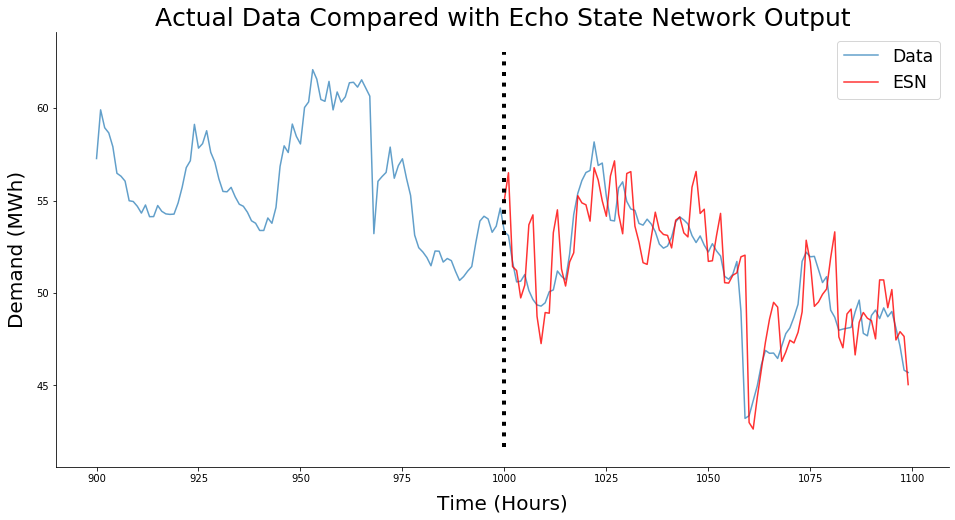
\includegraphics[width=\columnwidth]{scaled_esn_network2.png}
  \caption{A simple ESN with a prediction of 100 hours into the future after
  training on 1000 hours of historical data.}
  \label{fig:ESN1}
\end{figure}
\begin{figure}[h]
  \centering
  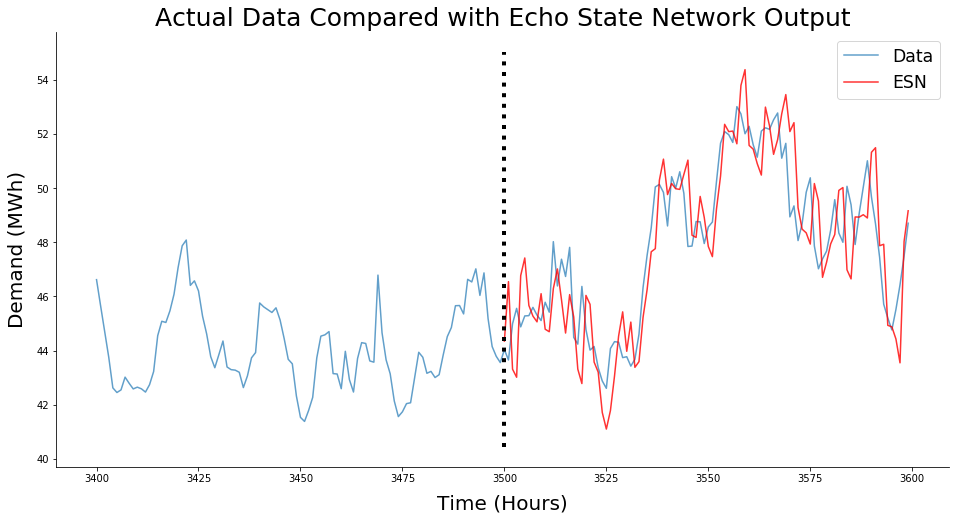
\includegraphics[width=\columnwidth]{scaled_esn_network.png}
  \caption{A simple ESN with a prediction of 100 hours into the future. After
  training on 3500 hours of historical data.}
  \label{fig:ESN2}
\end{figure}
\begin{figure}[h]
  \centering
  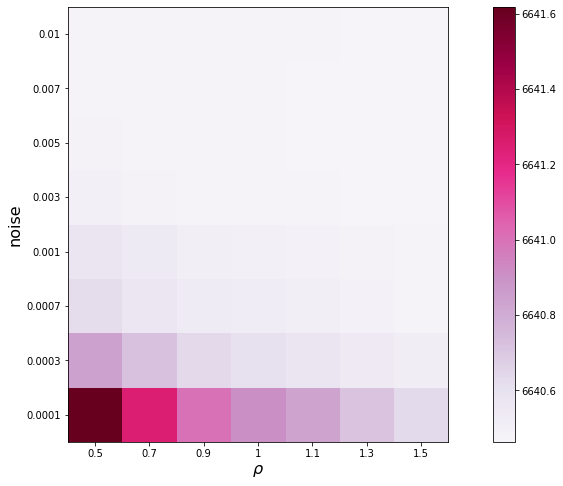
\includegraphics[width=0.8\columnwidth]{noise_spectral_radius.png}
  \caption{A grid search over a range of spectral radii and noise levels. The
  optimal set minimizes the mean squared error.}
  \label{fig:gridsearch}
\end{figure}
